\section{Data Formats\label{data_formats}}

In this section we describe the matrix and vector formats used internally by
\Az{}. 
In Section~\ref{highlevel_data_inter} we discuss a tool that transforms
data from a simpler format to this format. Here, the terms ``element'' and
``component'' are used interchangeably to denote a particular entry of a
vector.
User's who wish to supply their
own matrix-vector product can skip the matrix description and instead
read Section~\ref{matrix.free} where \Az{}'s matrix-free interface
is discussed.


The sparse matrix-vector product, $y \leftarrow Ax$, is the major kernel
operation of \Az{}. To perform this operation in parallel, the vectors $x$ and
$y$ as well as the matrix $A$ must be distributed across the processors.  The
elements of any vector of length $n$ are assigned to a particular processor via
some partitioning method (e.g. {\bf Chaco}~\cite{chaco}).  When calculating
elements in a vector such as $y$, a processor computes only those elements in
$y$ which it has been assigned.  These vector elements are explicitly stored on
the processor and are defined by a set of indices referred to as the
processor's {\it update\/} set.  The {\it update\/} set is further divided into
two subsets: {\it internal} and {\it border}.  A component corresponding to an
index in the {\it internal} set is updated using only information on the
current processor.  As an example, the index $i$ is in {\it internal} if, in
the matrix-vector product kernel, the element $y_i$ is updated by this
processor and if each $j$ defining a nonzero $A_{ij}$ in row $i$ is in {\it
  update\/}.  The {\it border} set defines elements which would require values
from other processors in order to be updated during the matrix vector product.
For example, the index $i$ is in {\it border} if, in the matrix-vector product
kernel, the element $y_i$ is updated by this processor and if there exists at
least one $j$ associated with a nonzero $A_{ij}$ found in row $i$ that is not
in {\it update\/}.  In the matrix-vector product, the set of indices which
identify the off-processor elements in $x$ that are needed to update components
corresponding to {\it border} indices is referred to as {\it external}.  They
are explicitly stored by and are obtained from other processors via
communication whenever a matrix-vector product is performed.
Figure~\ref{aztec_decomp} illustrates how a set of vertices in a partitioning
of a grid would be used to define these sets.
\begin{figure}[Htbp]
  \shadowbox{
%    \begin{minipage}{\textwidth}
    \begin{minipage}{6.2in}
      \vspace{0.5em}
  \centerline{\epsfig{file=./figs/aztec_decomp.eps,height=4.5in,clip}}
      \vspace{0.5em}
    \end{minipage}}
  \caption{Example partitioning of a finite element grid.} \label{aztec_decomp}
\end{figure}
Since these sets of indices are used exclusively to reference specific vector
components, the same names (i.e., {\it update\/}, {\it internal\/}, {\it
  border\/} and {\it external\/}) are sometimes used below to describe the
vector elements themselves.  Having generalized these labels, the three types
of vector elements are distinguished by locally storing the {\it internal}
components first, followed by the {\it border} components and finally by the
{\it external} components.  In addition, all {\it external} components received
from the same processor are stored consecutively.  Below we summarize the
nomenclature for a processor with $N$ total elements where {\it N\_internal\/},
{\it N\_border\/}, and {\it N\_external\/} elements are distributed over the
sets {\it internal\/}, {\it border\/} and {\it external\/} respectively.
\vskip .2in
\begin{center}
  \begin{tabularx}{\textwidth}{|l|X|X|} \hline
    \bf set & \bf description & \bf local numbering \\ \hline \hline
    \it internal & updated w/o communication & $0$ to $ N\_internal - 1$.\\
    \hline
    \it border & updated with communication & $N\_internal$ to $N\_internal
    + N\_border - 1$. \\ \hline
    \it external & not updated but used to update \it border. & $N\_internal +
    N\_border$ to $N - 1$. Elements received from the same processor are
    numbered consecutively. \\ \hline
  \end{tabularx}
\end{center}
\vskip .2in

Similar to vectors, a subset of matrix non-zeros is stored on each processor.
In particular, each processor stores only those rows which correspond to its
{\it update\/} set.  For example, if vector element $i$ is updated on processor
$p$, then processor $p$ also stores all the non-zeros of row $i$ in the matrix.
Further, the local numbering of vector elements on a specific processor induces
a local numbering of matrix rows and columns.  For example, if vector element
$k$ is locally numbered as $k_l$, then all references to row $k$ or column $k$
in the matrix would be locally numbered as $k_l$.  Thus, each processor
contains a submatrix whose row and column entries correspond to variables
defined on this processor.

The remainder of this section describes the two sparse matrix formats that are
used to store the local renumbered submatrix. These two sparse matrix formats
correspond to common formats used in serial computations.

\subsection{Distributed Modified Sparse Row (DMSR) Format} \label{DMSR Format}

The DMSR format is a generalization of the MSR format~\cite{concurrency}. The
data structure consists of an integer vector {\it bindx\/} and a double
precision vector {\it val\/} each of length {\it N\_nonzeros + 1} where {\it
  N\_nonzeros} is the number of nonzeros in the local submatrix.  For a
submatrix with $m$ rows the DMSR arrays are as follows:
%
\vspace{2em}
%{\flushleft{\bf Descriptions} \hrulefill}
%\nopagebreak% \\[0.5em]
\begin{tabbing}
$\hphantom{rp}$
\= {\it bindx {\bf :}\/} \\[0.3em]
\>$\hphantom{rpntrsqv}$
  \= {\it bindx[0]\/} \hskip 0.9in \= = \= m + 1 \\
\>\> {\it bindx[k+1] - bindx[k]\/} \> = \> number of nonzero
                                           off-diagonal elements
                                           in {\it k\/}'th \\
\>\>                               \>   \> row, $k < m $ \\
\>\> {\it bindx[$k_s ... k_e$]\/}  \> = \> column indices of the
                                           off-diagonal
                                           nonzeros in row\\
\>\>                               \>   \> $k$ where
                                           $k_s$ = {\it bindx[k]} and
                                           $k_e$ = {\it bindx[k+1]-1}.\\[0.8em]
\> {\it val {\bf :}\/} \\[0.3em]
\>\> {\it val[k] \/}               \> = \> $ A_{kk}, k < m $ \\
\>\> {\it val[$k_i$] \/}   \> = \> the ($k$, {\it bindx[$k_i$] \/})'th
                                           matrix element where \\
\>\>                               \>   \> $k_s \leq k_i \leq k_e $
                                           with $k_s$ and $k_e$ as defined
                                           above.
\end{tabbing}
%
\vspace{1em}
Note: {\it val[m]\/} is not used. See~\cite{sparker2} for a detailed
discussion of the MSR format.

\subsection{Distributed Variable Block Row (DVBR) Format} \label{DVBR Format}

The Distributed Variable Block Row (DVBR) format is a generalization of the VBR
format~\cite{sparker2}.  The data structure consists of a double precision
vector {\it val\/} and five integer vectors: {\it indx\/}, {\it bindx\/}, {\it
  rpntr\/}, {\it cpntr\/} and {\it bpntr\/}.  The format is best suited for
sparse block matrices of the form
\[
A = \left( \begin{array}{cccc}
        A_{00} & A_{01} & \cdots & A_{0k} \\
        A_{10} & A_{11} & \cdots & A_{1k} \\
        \vdots & & \ddots & \vdots \\
        A_{m0} & \cdots & \cdots & A_{mk} \end{array}
\right)
\]
where $A_{ij}$ denotes a block (or submatrix). In a sparse block matrix, some
of these blocks would be entirely zero while others may be dense. The DVBR
vectors are described below for a matrix with $M \times K$ blocks.
%
\vspace{1em}
%{\flushleft{\bf Descriptions} \hrulefill}
%\nopagebreak %\\[0.5em]
\begin{tabbing}
$\hphantom{rp}$
\= {\it rpntr[0 ... M] {\bf :}\/} \\[0.3em]
\>$\hphantom{rpntrsqv}$
  \= {\it rpntr[0]\/} \hskip 0.9in \= = \= 0 \\
\>\> {\it rpntr[k+1] - rpntr[k]\/} \> = \> number of rows in {\it
                                           k\/}'th block row \\[0.8em]
\> {\it cpntr[0 ... K] {\bf :}\/} \\[0.3em]
\>\> {\it cpntr[0]\/}              \> = \> 0 \\
\>\> {\it cpntr[k+1] - cpntr[k]\/} \> = \> number of columns in {\it
                                           k\/}'th block column \\[0.8em]
\> {\it bpntr[0 ... M] {\bf :}\/} \\[0.3em]
\>\> {\it bpntr[0]\/}              \> = \> 0 \\
\>\> {\it bpntr[k+1] - bpntr[k]\/} \> = \> number of nonzero blocks in the
                                           {\it k\/}'th block row\\[0.8em]
\> {\it bindx[0 ... bpntr[M] - 1] {\bf :}\/}\\[0.3em]
\>\> {\it bindx[$k_s ... k_e$]\/}  \> = \> block column indices of nonzero
                                           blocks in block row $k$ \\
\>\>                               \>   \> where $k_s$ = {\it bpntr[k]} and
                                           $k_e$ = {\it bpntr[k+1]}-1 \\[0.8em]
\> {\it indx[0 ... bpntr[M] ] {\bf :}\/}\\[0.3em]
\>\> {\it indx[0]\/}               \> = \> 0 \\
\>\> {\it indx[$k_i$+1] - indx[$k_i$]\/}\> = \> number of nonzeros in
                                                the ($k$, {\it
                                                bindx[$k_i$]\/})'th
                                                block \\
\>\>                               \>   \> where $k_s \leq k_i \leq
                                           k_e$ with $k_s$ and $k_e$
                                           as defined \\
\>\>                               \>   \> above. \\[0.8em]
\> {\it val[0 ... indx[bpntr[M]] - 1 ] {\bf :}\/}\\[0.3em]
\>\> {\it val[$i_s ... i_e$]\/}  \> = \> nonzeros in the ($k$, {\it
     bindx[$k_i$]\/})'th block stored in \\
\>\>                             \>   \> column major order where
                                         $k_i$ is as defined above, \\
\>\>                             \>   \> $i_s$ = {\it indx[$k_i$]} and
                                         $i_e$ = {\it indx[$k_i$+1]}-1
\end{tabbing}
\vspace{1em}
%
See~\cite{sparker2} for a detailed discussion of the VBR format.

%%% Local Variables:
%%% mode: latex
%%% TeX-master: "az_ug_20"
%%% End:
